
\documentclass{beamer}

\usepackage{algpseudocode, color, colortbl}

\usepackage{hyperref}
\hypersetup{
    colorlinks=true,
    urlcolor=blue,
}

\usepackage{listings}

\usepackage{tikz}

\usetheme{Montpellier}
\usecolortheme{rose}

% page numbers, from
% https://tex.stackexchange.com/questions/137022/how-to-insert-page-number-in-beamer-navigation-symbols
\expandafter\def\expandafter\insertshorttitle\expandafter{%
  \insertshorttitle\hfill%
  \insertframenumber\,/\,\inserttotalframenumber}

\definecolor{Gray}{gray}{0.8}
\newcolumntype{g}{>{\columncolor{Gray}}c}

\newcommand{\stanza}{ \\~\ }

\title{09. Bipartite Matching}
\subtitle{CPSC 535}
\author{Kevin A. Wortman}
\institute{ 
\includegraphics[height=2cm]{csuf-logo-cmyk} }
\date{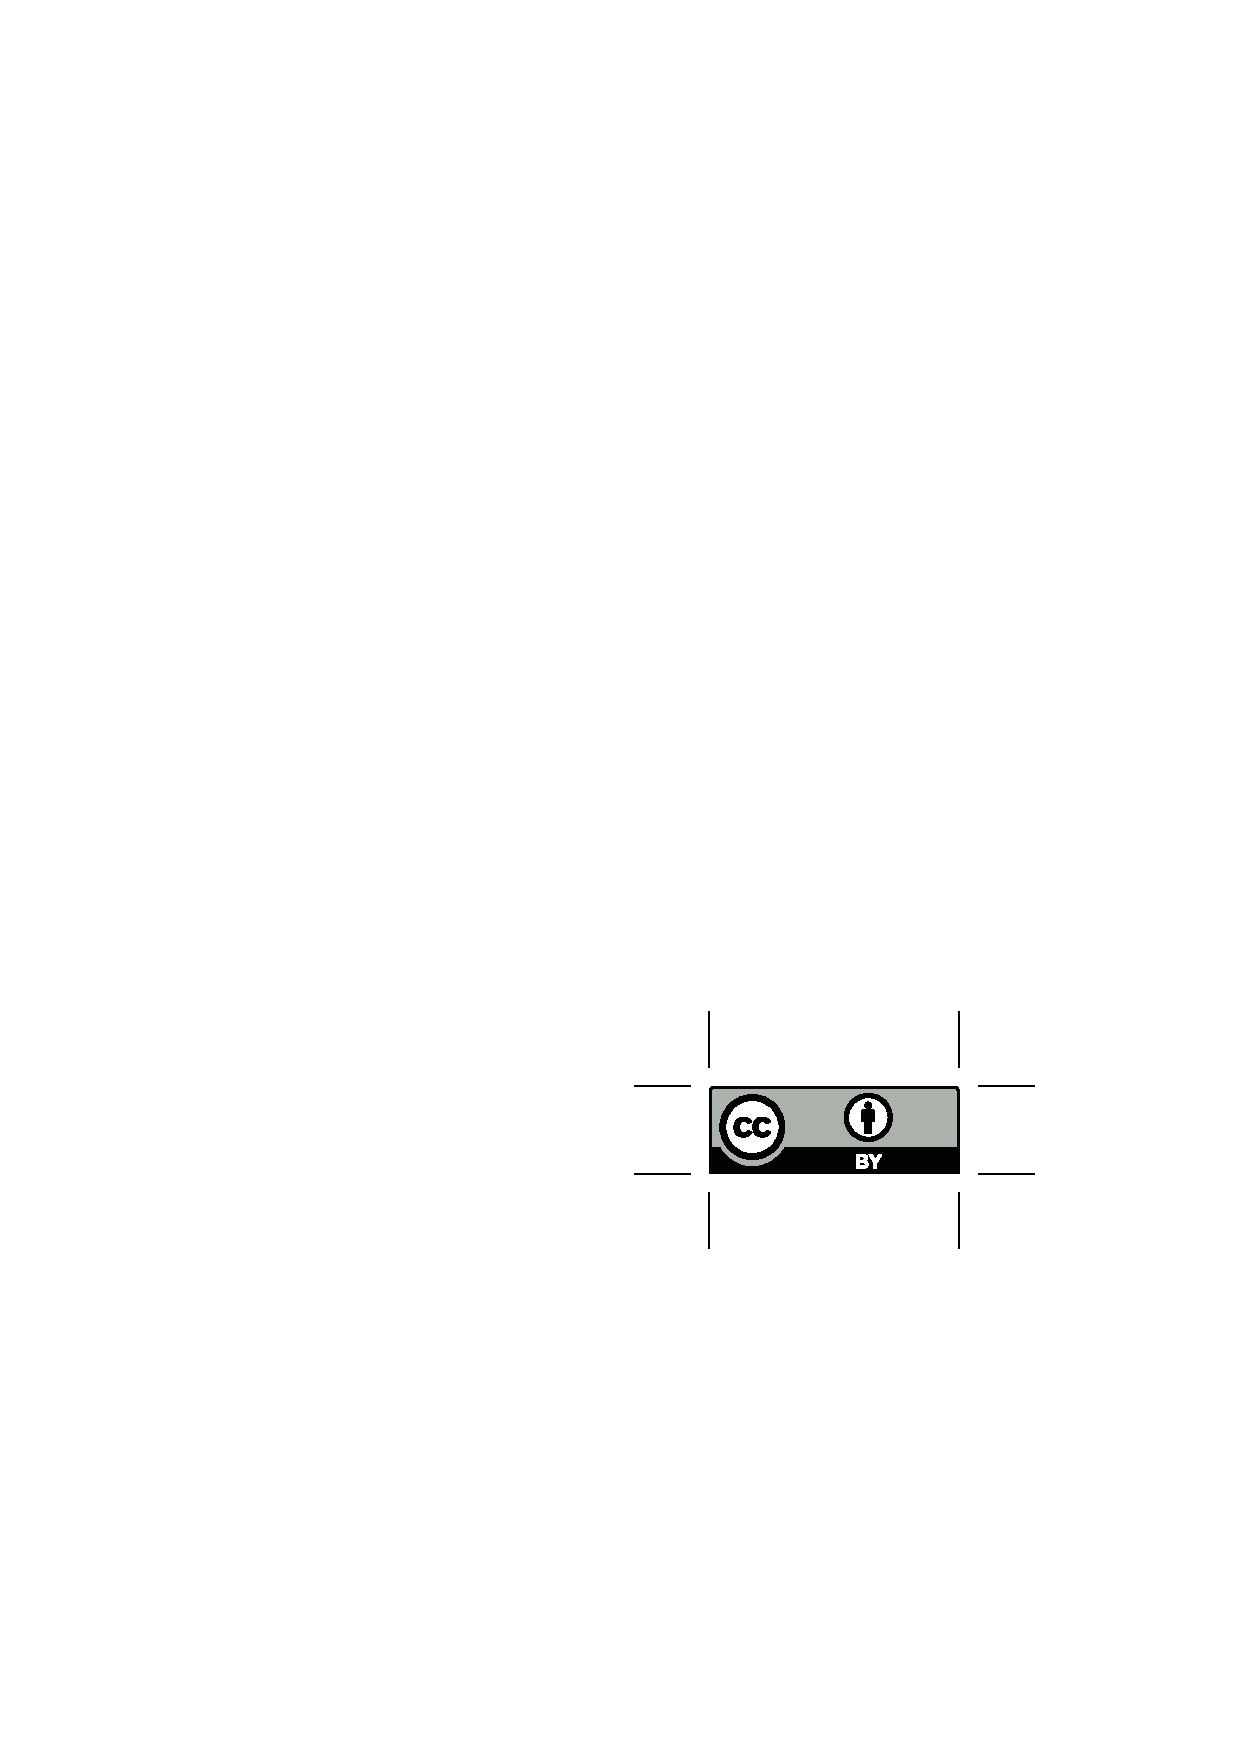
\includegraphics[height=14pt]{by} \\

{\tiny
This work is licensed under a
\href{http://creativecommons.org/licenses/by/4.0/}{Creative Commons Attribution 4.0 International License}.
}}

\begin{document}

\begin{frame}
  \titlepage
\end{frame}

\begin{frame} \frametitle{Bipartite Matching}
So far, all our reductions to max-flow have been either straightforward
flow simulations, or variations on max-flow. \stanza

Now we'll see a quite-different problem that also reduces to max-flow.
\end{frame}

\begin{frame} \frametitle{Partition of a Set}

  Intuitively: if $X = L \cup R$ is a \emph{partition,} then every element of $X$ is placed in $L$ or $R$ (but not both). \stanza

  Formally: $L$ and $R$ partition $X$ if
  \begin{itemize}
  \item $X = L \cup R,$
  \item $L \cap R = \emptyset,$ and
  \item $L \ne \emptyset, R \ne \emptyset.$
  \end{itemize}
  
\end{frame}

\begin{frame} \frametitle{Bipartite Matching}
\textbf{bipartite maximum matching} \\
\emph{input:} an undirected bipartite graph $G=(V, E)$ with parts $V=L \cup R$ \\
\emph{output:} a matching $M \subseteq E$ where the number of matched vertices
  is maximum \stanza

\begin{itemize}
  \item \emph{bipartite:} $L, R$ are disjoint and edges only go between $L, R$
  \item \emph{matching:} pick edges that ``pair off'' two vertices; goal is to
    maximize \#paired-off
  \item intuitively, $L$ is one kind of thing and $R$ is another kind of thing
\end{itemize}
\end{frame}

\begin{frame} \frametitle{Bipartite Matching}
\begin{center}
  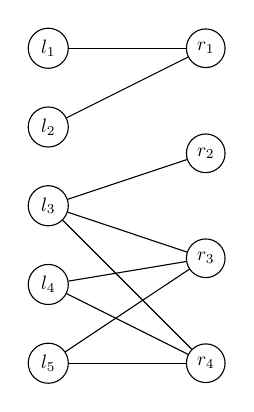
\begin{tikzpicture}[every node/.style={scale=.7}]

    \node [draw, circle] (l1) at (0, 4) {$l_1$};
    \node [draw, circle] (l2) at (0, 3) {$l_2$};
    \node [draw, circle] (l3) at (0, 2) {$l_3$};
    \node [draw, circle] (l4) at (0, 1) {$l_4$};
    \node [draw, circle] (l5) at (0, 0) {$l_5$};

    \node [draw, circle] (r1) at (2, 4) {$r_1$};
    \node [draw, circle] (r2) at (2, 2.666) {$r_2$};
    \node [draw, circle] (r3) at (2, 1.333) {$r_3$};
    \node [draw, circle] (r4) at (2, 0) {$r_4$};

    \draw (l1) to (r1);
    \draw (l2) to (r1);

    \draw (l3) to (r2);
    \draw (l3) to (r3);
    \draw (l3) to (r4);

    \draw (l4) to (r3);
    \draw (l4) to (r4);

    \draw (l5) to (r3);
    \draw (l5) to (r4);

  \end{tikzpicture}
\end{center}
\end{frame}

\begin{frame} \frametitle{Bipartite Matching}
\begin{center}
  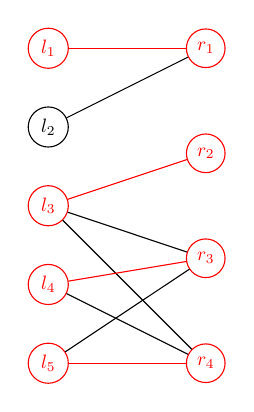
\begin{tikzpicture}[every node/.style={scale=.7}]

    \node [draw, circle, color=red] (l1) at (0, 4) {$l_1$};
    \node [draw, circle] (l2) at (0, 3) {$l_2$};
    \node [draw, circle, color=red] (l3) at (0, 2) {$l_3$};
    \node [draw, circle, color=red] (l4) at (0, 1) {$l_4$};
    \node [draw, circle, color=red] (l5) at (0, 0) {$l_5$};

    \node [draw, circle, color=red] (r1) at (2, 4) {$r_1$};
    \node [draw, circle, color=red] (r2) at (2, 2.666) {$r_2$};
    \node [draw, circle, color=red] (r3) at (2, 1.333) {$r_3$};
    \node [draw, circle, color=red] (r4) at (2, 0) {$r_4$};

    \draw [color=red] (l1) to (r1);
    \draw (l2) to (r1);

    \draw [color=red] (l3) to (r2);
    \draw (l3) to (r3);
    \draw (l3) to (r4);

    \draw [color=red] (l4) to (r3);
    \draw (l4) to (r4);

    \draw (l5) to (r3);
    \draw [color=red] (l5) to (r4);

  \end{tikzpicture}

  matching $M = \{\text{included edges}\}
    = \{ \{l_1, r_1\}, \{l_3, r_3\}, \{l_4, r_3\}, \{l_5, r_4\} \}$ \\

    $|M|=4$ \\

    (other optimal matchings exist)
\end{center}
\end{frame}

\begin{frame} \frametitle{Bipartite Matching Applications}
\begin{itemize}
  \item any scenario where there are two kinds of things that can be paired
  \item goal is simply maximum number of pairings
  \item casting for a play: $L = $ set of actors; $R = $ set of roles;
    edge $\{l, r\}$ exists when $l$ could play role $r$
  \item packing leftover food (one item/container): $L = $ set of food items; $R = $ available
    containers; edge $\{l, r\}$ exists when food $l$ could fit in container $r$
  \item scheduling appointments: $L = $ set of clients; $R = $ set of time slots;
    edge $\{l, r \}$ exists when client $l$ could meet appointment $r$
  \item might feel $NP$-hard, but actually in $P$
\end{itemize}
\end{frame}

\begin{frame} \frametitle{Formulating Bipartite Matching as Flow}
\begin{itemize}
  \item let $G=(V, E)$ be bipartite matching instance
  \item create $G'=(V', E')$ with $V' = V \cup \{s, t\}$ where $s, t$ are new
    source/sink
  \item create edges in $G'$:
  \begin{itemize}
    \item $(l, r) \enspace \forall l \in L, r \in R, \{l, r\} \in E$
    \item $(s, l) \enspace \forall l \in L$
    \item $(r, t) \enspace \forall r \in R$
  \end{itemize}
  \item every edge $(v, w)$ has capacity $c(v, w)=1$
  \item post-processing: edge $(l, r) \in M$ iff $f(l, r)=1$
  \item observe $|V'| \in O(|V|), |E'| \in O(|E|),$ overhead is $O(|V|+|E|)$
  \item $\implies$ if this is correct, can solve bipartite matching in $O(|V|^3)$ time
\end{itemize}
\end{frame}

\begin{frame} \frametitle{Formulating Bipartite Matching as Flow}
  \begin{center}
  \begin{tabular}{cccc}
  $G$ & $G'$ & $f'$ & $M$ \\

  % G
  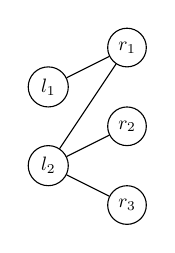
\begin{tikzpicture}[every node/.style={scale=.7}]
    \node [draw, circle] (l1) at (0, 1.5) {$l_1$};
    \node [draw, circle] (l2) at (0, .5) {$l_2$};
    \node [draw, circle] (r1) at (1, 2) {$r_1$};
    \node [draw, circle] (r2) at (1, 1) {$r_2$};
    \node [draw, circle] (r3) at (1, 0) {$r_3$};
    \draw (l1) to (r1);
    \draw (l2) to (r1);
    \draw (l2) to (r2);
    \draw (l2) to (r3);
  \end{tikzpicture}

  % G'
  &
  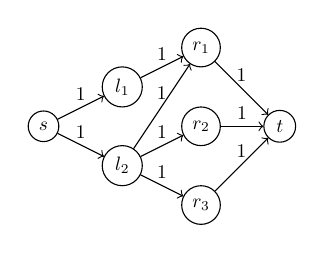
\begin{tikzpicture}[every node/.style={scale=.7}]
    \node [draw, circle] (l1) at (0, 1.5) {$l_1$};
    \node [draw, circle] (l2) at (0, .5) {$l_2$};
    \node [draw, circle] (r1) at (1, 2) {$r_1$};
    \node [draw, circle] (r2) at (1, 1) {$r_2$};
    \node [draw, circle] (r3) at (1, 0) {$r_3$};

    \node [draw, circle] (s) at (-1, 1) {$s$};
    \node [draw, circle] (t) at (2, 1) {$t$};

    \draw [->] (l1) to node [above] {1} (r1);
    \draw [->] (l2) to node [above] {1} (r1);
    \draw [->] (l2) to node [above] {1} (r2);
    \draw [->] (l2) to node [above] {1} (r3);

    \draw [->] (s) to node [above] {1} (l1);
    \draw [->] (s) to node [above] {1} (l2);
    \draw [->] (r1) to node [above] {1} (t);
    \draw [->] (r2) to node [above] {1} (t);
    \draw [->] (r3) to node [above] {1} (t);
  \end{tikzpicture}

  % f'
  &
  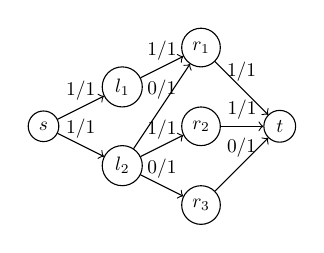
\begin{tikzpicture}[every node/.style={scale=.7}]
    \node [draw, circle] (l1) at (0, 1.5) {$l_1$};
    \node [draw, circle] (l2) at (0, .5) {$l_2$};
    \node [draw, circle] (r1) at (1, 2) {$r_1$};
    \node [draw, circle] (r2) at (1, 1) {$r_2$};
    \node [draw, circle] (r3) at (1, 0) {$r_3$};

    \node [draw, circle] (s) at (-1, 1) {$s$};
    \node [draw, circle] (t) at (2, 1) {$t$};

    \draw [->] (l1) to node [above] {1/1} (r1);
    \draw [->] (l2) to node [above] {0/1} (r1);
    \draw [->] (l2) to node [above] {1/1} (r2);
    \draw [->] (l2) to node [above] {0/1} (r3);

    \draw [->] (s) to node [above] {1/1} (l1);
    \draw [->] (s) to node [above] {1/1} (l2);
    \draw [->] (r1) to node [above] {1/1} (t);
    \draw [->] (r2) to node [above] {1/1} (t);
    \draw [->] (r3) to node [above] {0/1} (t);
  \end{tikzpicture}

    % M
    &
    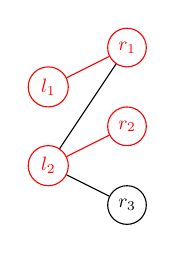
\begin{tikzpicture}[every node/.style={scale=.7}]
      \node [draw, circle, color=red] (l1) at (0, 1.5) {$l_1$};
      \node [draw, circle, color=red] (l2) at (0, .5) {$l_2$};
      \node [draw, circle, color=red] (r1) at (1, 2) {$r_1$};
      \node [draw, circle, color=red] (r2) at (1, 1) {$r_2$};
      \node [draw, circle] (r3) at (1, 0) {$r_3$};
      \draw [color=red] (l1) to (r1);
      \draw (l2) to (r1);
      \draw [color=red] (l2) to (r2);
      \draw (l2) to (r3);
    \end{tikzpicture}

  \end{tabular}
  \vspace{.5cm}
  $M = \{ \{l, r\} \, | \, f'(l, r)=1 \} = \{ \{l_1, r_1\}, \{l_2, r_2\} \}$ \\
  (other max flows $\Leftrightarrow$ matchings exist)
  \end{center}
\end{frame}

\begin{frame} \frametitle{Correctness of this Formulation}
Technical details:
\begin{itemize}
  \item \emph{integrality theorem:} if every capacity $c(u, v) \in \mathbb{Z}$
    then every $f(u, v) \in \mathbb{Z}$ and $|f| \in \mathbb{Z}$
  \item $\exists$ matching $M$ with cardinality $k=|M|$ iff $\exists$ some flow $f$
    with value $k=|f|$
    \begin{itemize}
      \item key idea: pairing two vertices in the matching adds exactly one
        flow from $s \leadsto t$
      \item there are no opportunities for flow aside from matched vertices
    \end{itemize}
  \item $\implies$ a maximum flow in $G'$ corresponds to a maximum matching in $G$
\end{itemize}
\end{frame}

\begin{frame} \frametitle{Summary}
  \begin{itemize}
    \item classical max-flow problem can be solved in $O(|V|^3)$ time, in $P$
    \item robust max-flow problem (supports unreachable vertices, antiparallel edges, multiple sinks/sources)
      also in $O(|V|^3)$ time w/ worse constant factors, in $P$
    \item bipartite matching reduces to max-flow, so bipartite matching can be solved in
      $O(|V|^3)$ time, in $P$
    \item other practical, distinct problems reduce to max-flow or bipartite
      matching so take $O(|V|^3)$ time and are in $P$
  \end{itemize}
\end{frame}

\end{document}
